\scanpage{7}
\deleted{\illegible{1}} Let $a\in\mathbb N^*,b\in\mathbb N^*,c\in\mathbb N^*,\ q\in\mathbb N^*$ \quad $q$ a prime number $(q\ne1)$

We assume that $a\mathrel{\underset{1}{\smile}}b$, $a\mathrel{\underset{1}{\smile}}c$, $b\mathrel{\underset{1}{\smile}}c$ (pairwise relatively prime)
\inserted{and $a^q+b^q=c^q$}

We have $c>a$ and $c>b$ since $a\in\mathbb N^*$ and $b\in\mathbb N^*$

We put $c=a+b'=b+a'$ with $b'\in\mathbb N^*$ and $a'\in\mathbb N^*$
\[
\begin{aligned}
\text{then}\qquad a^q+b^q=c^q&=(a+b')^q=\sum_{i=0}^{q}C_q^i\,a^i b'^{\,q-i}\qquad\text{(Newton)}\\
 &=b'^{\,q}+\sum_{i=1}^{q-1}C_q^i\,a^i b'^{\,q-i}+a^q\qquad(\text{since }q\geqslant2)
\end{aligned}
\]
\[
\text{thus}\qquad b^q=\sum_{i=1}^{q-1}C_q^i\,a^i b'^{\,q-i}+b'^{\,q}\tag*{(1)}
\]
the power of $b'$ never being zero we can factor out $b'$ on the right-hand side of (1), thus $b'\mid b^q$ ($b'$ divides $b^q$)

Let $p$ be a prime number % The phrase is visibly drawn once by rlap. The phantom preserves its deletion
% annotation and text dimensions without adding the generic horizontal rule.
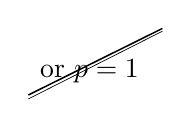
\begin{tikzpicture}[baseline=(cancelled.base)]
\node[inner sep=0pt,outer sep=0pt] (cancelled)
 {\rlap{or $p=1$}\phantom{\deleted{or $p=1$}}};
\draw[line width=.55pt] ([xshift=-1.5mm,yshift=-1.5mm]cancelled.south west) -- ([xshift=3mm,yshift=4mm]cancelled.north east);
\draw[line width=.25pt] ([xshift=-1.5mm,yshift=-2mm]cancelled.south west) -- ([xshift=3mm,yshift=3.65mm]cancelled.north east);
\end{tikzpicture}
 and such that : $p\mid b'$ thus $p\mid b$. Let $\alpha\in\mathbb N^*$ and $\alpha'\in\mathbb N^*$ be such that
\[
\begin{aligned}
 &p^{\alpha'}\mid b'\quad\text{and}\quad p^{\alpha'+1}\nmid b'\\
 \text{and}\quad &p^\alpha\mid b\quad\text{and}\quad p^{\alpha+1}\nmid b
\end{aligned}
\]
\margin{$\unsure{a|\alpha}$ \unsure{does not exist|does not exist} if we had $p=1$}
We have $\alpha'\leqslant q\alpha$ since $b'\mid b^q$

\[
\begin{aligned}
(1)\ \Longrightarrow\quad&p^{q\alpha}\mid\sum_{i=1}^{q-1}C_q^i\,a^i b'^{\,q-i}+b'^{\,q}\\
\Longrightarrow\quad&p^{q\alpha}\mid b'\left(\sum_{i=1}^{q-1}C_q^i\,a^i b'^{\,q-i-1}+b'^{\,q-1}\right)\qquad(\text{since }q\geqslant2)
\end{aligned}
\]
let us put $b'=p^{\alpha'}b''$ thus $b''\mathrel{\underset{1}{\smile}}p$ (property of $\alpha'$)
\[
\begin{aligned}
\Longrightarrow\quad&p^{q\alpha}\mid p^{\alpha'}b''\left(\sum_{i=1}^{q-1}C_q^i\,a^i b'^{\,q-i-1}+b'^{\,q-1}\right)\\
\Longrightarrow\quad&p^{q\alpha-\alpha'}\mid b''\left(\sum_{i=1}^{q-1}C_q^i\,a^i b'^{\,q-i-1}+b'^{\,q-1}\right)\quad\text{since }q\alpha\geqslant\alpha'\\
\Longrightarrow\quad&p^{q\alpha-\alpha'}\mid\sum_{i=1}^{q-1}C_q^i\,a^i b'^{\,q-i-1}+b'^{\,q-1}\quad\text{since }b''\mathrel{\underset{1}{\smile}}p
\end{aligned}
\]
% archive sheet number: 6
